O principal componente do TinyOS, responsável por inicializar o sistema, é chamado \textit{MainC}. 
Ele inicializa os componentes de hardware e software e o escalonador de tarefas. Para isso, \textit{MainC} se liga aos
componentes \textit{RealmainP}, \textit{PlataformC}, \textit{TinySchedulerC}, e utiliza a interface \textit{SoftwareInit}.

\begin{figure}[htb]
\centering
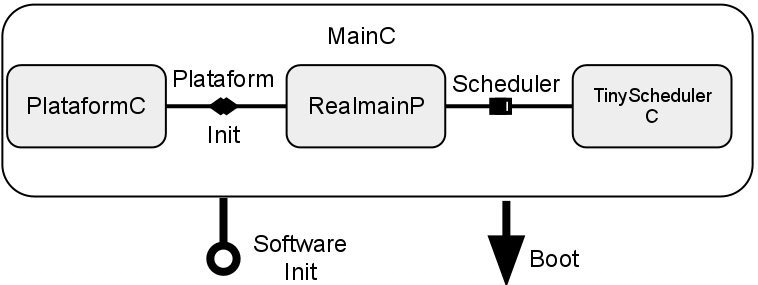
\includegraphics[scale=0.4]{images/mainc.png}
\caption{MainC}
\end{figure}

Primeiro é configurado o sistema de memória e escolhido o modo de processamento. 
Com esses pré-requisitos básicos estabelecidos,  o escalonador de tarefas é inicializado 
para permitir que as próximas etapas possam postar tarefas.
O segundo passo é inicializar os demais componentes de hardware, permitindo a operabilidade da plataforma.
Alguns exemplos são configuração de pinos de entrada e saída, calibração do clock e dos LEDs.
Como esta etapa exige códigos específicos para cada tipo de plataforma, o MainC se liga ao componente
\textit{PlataformC} que implementa o tratamento requerido por cada tipo de plataforma.

\begin{figure}[htb]
\centering
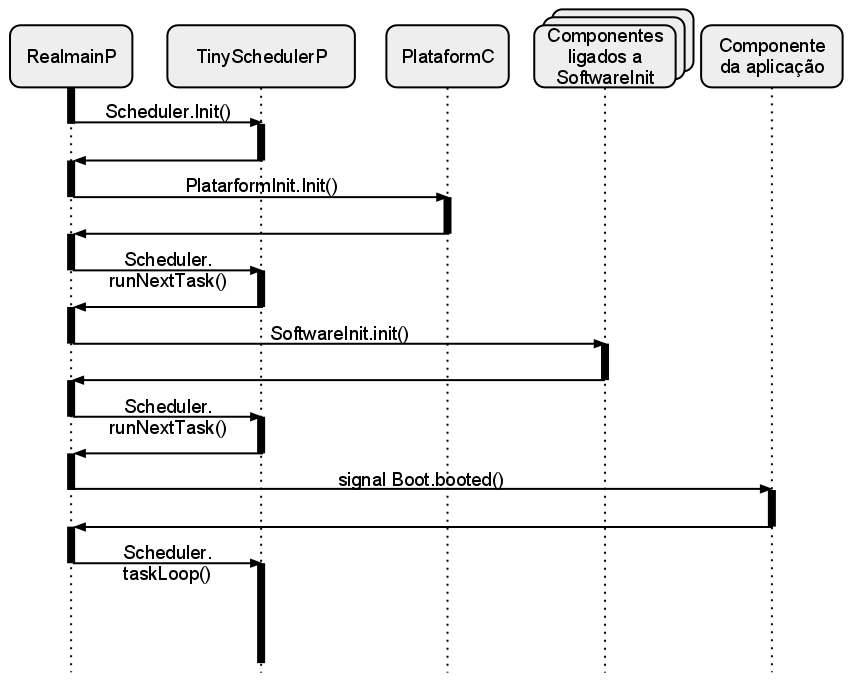
\includegraphics[scale=0.45]{images/sequencia-de-inicializacao.png}
\caption{Sequência de Inicialização}
\end{figure}

O terceiro passo trata da inicialização dos componentes de software. 
Além de configurar os aplicativos básicos do sistema, como
os \textit{timer}s, nesta etapa são executados também os procedimentos de inicialização dos componentes 
da aplicação. Para isso, os componentes da aplicação que precisam ser inicializados devem oferecer a interface
{\em SoftwareInit}. Assim, durante a etapa de inicialização do sistema, os códigos de inicialização dos componentes da
aplicação são automaticamente chamados.
% !!! Esse paragrafo a cima parece ter muito a palavra inicialização !!!

Por último, quando todas as etapas foram concluídas, o MainC avisa a aplicação que a inicialização terminou, através do
evento \textit{Boot.booted()}. O TinyOS entra no
seu laço principal, no qual o escalonador espera por tarefas e as executa. É importante notar que
durante todo o processo de inicialização as interrupções do sistema ficam desabilitadas~\cite{TEP107}.

\begin{lstlisting}[caption=Código de inicialização]
module RealMainP {
    provides interface Booted;
    uses {
        interface Scheduler;
        interface Init as PlatformInit;
        interface Init as SoftwareInit;
    }
}
implementation {
     int main() __attribute__ ((C, spontaneous)) {
         atomic {
             platform_bootstrap();
             call Scheduler.init();
             call PlatformInit.init();
             while (call Scheduler.runNextTask());
             call SoftwareInit.init();
             while (call Scheduler.runNextTask());
         }
         __nesc_enable_interrupt();
         signal Boot.booted();
         call Scheduler.taskLoop();
         return -1;
     }
 \end{lstlisting}

